\chapter{Introduction}

\graphicspath{{./Figures/Introduction/}}



\section{Motivation}
%This section should explore the underlying reasons for undertaking the research. It might include the importance of the topic, the gap in current knowledge, and the potential applications of the research findings.
%figure for Handle Boston Dynamics Robot
\begin {figure}[h]
\centering
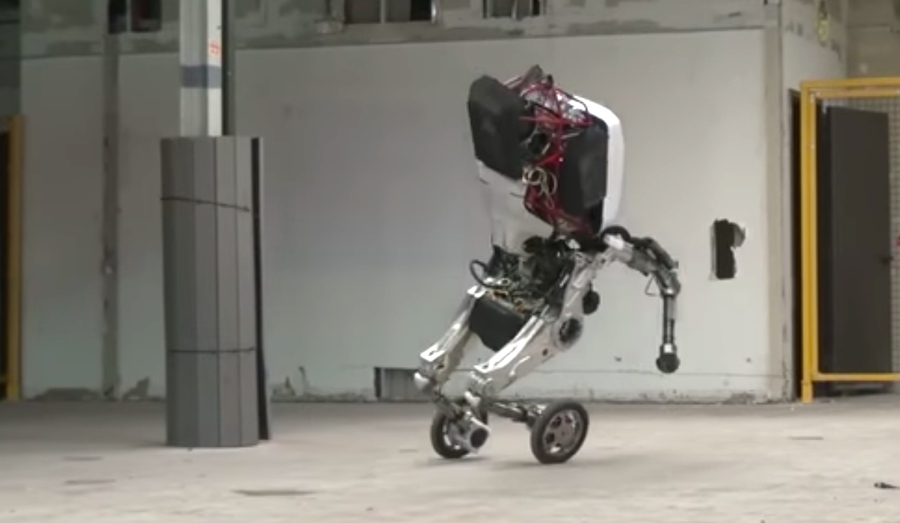
\includegraphics[width=0.7\textwidth]{boston-dynamics-handle-robot}
\caption{Handle Robot by Boston Dynamics\cite{handle}}
\label{fig:Handle}
\end {figure}


Robotics has always been a cutting-edge field that combines sophisticated engineering, artificial intelligence, and a comprehension of human-environment interactions.
This study is motivated by multiple important elements, all of which highlight the importance and relevance of the research.
The reasons for undertaking this research is the desire to advance the field of robotics, fill existing knowledge gaps, have a broad societal impact, and foster interdisciplinary collaboration.
By developing a multi-legged robotic system with enhanced movement capabilities and control strategies, this research endeavors to set new standards in robotic design and functionality. Even with significant advancements, there are still many unanswered questions about robotic control and locomotion, particularly in systems that replicate biological structures and processes. Complex dynamic tasks that living beings handle with ease are sometimes difficult for traditional robotic systems to accomplish. This research aims to close these gaps by concentrating on a multi-legged robot that finds inspiration in the natural environment. This will provide insights into more realistic and effective movement tactics. The applications of such advanced robotic systems are vast and varied, ranging from search and rescue operations in hazardous environments to assistive technology in warehouse automation.By pushing the boundaries of what is currently possible in robotic design and control, this research has the potential to make significant contributions to fields where human intervention is limited, dangerous, or impractical. This project is inherently interdisciplinary, integrating concepts from mechanical engineering, computer science, control theory, and even biology. Such cross-disciplinary collaboration is crucial for driving innovation, as it allows for the exchange of ideas and methods from diverse fields. This approach is expected to yield novel solutions and advancements that could extend well beyond the scope of this project.

%\textbf{Advancements in Robotic Technologies:}% Robotics has grown at an exponential rate over the past few decades, resulting in improved capabilities and more applications. Previously limited to industrial settings, robots are now being deployed in increasingly dynamic and unpredictable circumstances. The development of robotic systems that are more flexible, nimble, and intelligent is required due to this evolution. Our research is to create a sophisticated multi-legged robotic system that can perform intricate movements and interact with its surroundings.

%\textbf{Filling Knowledge Gaps:} %Even with significant advancements, there are still many unanswered questions about robotic control and locomotion, particularly in systems that replicate biological structures and processes. Complex dynamic tasks that living beings handle with ease are sometimes difficult for traditional robotic systems to accomplish. This research aims to close these gaps by concentrating on a multi-legged robot that finds inspiration in the natural environment. This will provide insights into more realistic and effective movement tactics.

%\textbf{Potential for Broad Impact:} %The applications of such advanced robotic systems are vast and varied, ranging from search and rescue operations in hazardous environments to assistive technology in healthcare. By pushing the boundaries of what is currently possible in robotic design and control, this research has the potential to make significant contributions to fields where human intervention is limited, dangerous, or impractical.

%\textbf{Interdisciplinary Collaboration and Innovation:} %This project is inherently interdisciplinary, integrating concepts from mechanical engineering, computer science, control theory, and even biology. Such cross-disciplinary collaboration is crucial for driving innovation, as it allows for the exchange of ideas and methods from diverse fields. This approach is expected to yield novel solutions and advancements that could extend well beyond the scope of this project.

%In summary, the motivation for this project lies in its potential to advance the field of robotics, fill existing knowledge gaps, have a broad societal impact, and foster interdisciplinary collaboration. By developing a multi-legged robotic system with enhanced movement capabilities and control strategies, this research endeavors to set new standards in robotic design and functionality.

\section{Explanation of the Goals and Requirements}
In this research, we aim to develop a multi-legged robotic system that can perform complex movements and interact with its environment.
The robot will be able to balance on two wheeled multi-jointed legs.
The robot would be based on the previous TWIPR robot.
Extra degrees of freedom will be added to the robot to allow for more complex movement.
The robot would be designed from scratch to meet the requirements of the project.
The robot would be designed using CAD software.
The design would take into account the mechanical, electrical, and software requirements of the robot.
Fabrication of the robot chassis would be done using 3D printing.Electrical design and assembly would be done using off-the-shelf components.
Mathematical modeling and simulation of the robot would be done to determine the robot's dynamics and control.
Different control strategies would be explored and implemented.
Development of firmware and software for the robot would be done.
The robot would be tested and evaluated in simulation and in real life.
The robot would be tested for its ability to balance and move in different environments. The robot would be tested for its ability to perform complex movements and interact with its environment.
